\section*{Mathematical Modelling and Methodology}
\hspace{\parindent}we aim to understand a particular phenomenon by presenting three mathematical models and conducting tests to determine the parameters of an ionic lifter. Additionally, we explore methods for optimizing the lifter's output and measuring its efficiency.
\subsection*{Models:}
The following are the three models considered:\\
1.\textbf{Ideal Case:}	 Infinite Plate and Infinite Wire\\
•	This model assumes an infinite grounded plate and an infinite wire with a negative voltage.\\
•	The wire has a radius of $r_o$ and is positioned at a distance of l cm from the plate.\\
•	When a high voltage is applied, electrons are discharged from the wire electrode, causing ionization of the surrounding air into negative ions.\\
•	These ions form a thin conducting layer, which is typically negligible.\\
•	Kaptzov's hypothesis states that the electric field on the surface of an electrode under corona discharge is constant, described by the equation: 
$$E_o = 3.1\times10^6(1 + \frac{0.308}{0.5r_c ^\frac{1}{2}}) V/m$$
where $r_c$ is the radius of curvature.\cite{sakr1}\\
2.\textbf{Classic Case:}	 Wire to Cylinder Lifter\\
 \hspace{\parindent}  In this model, the focus is on a wire formed circularly above the cathode. The processes of ion formation and force calculations are analyzed independently to gain a comprehensive understanding of their dynamics.\\
3.\textbf{Sharp Edges in the Wire:}	\\
•	This model explores the effect of introducing sharp edges to the wire.\\
•	The objective is to test whether the air ionization voltage is reduced.\\
\newpage 
\section*{Analysis}
\hspace{\parindent}For each of the models mentioned above, our analysis focuses on two aspects: the formation of ions and the forces acting on them.
\subsection*{Model 1: Infinite plane with a negative voltage wire}
%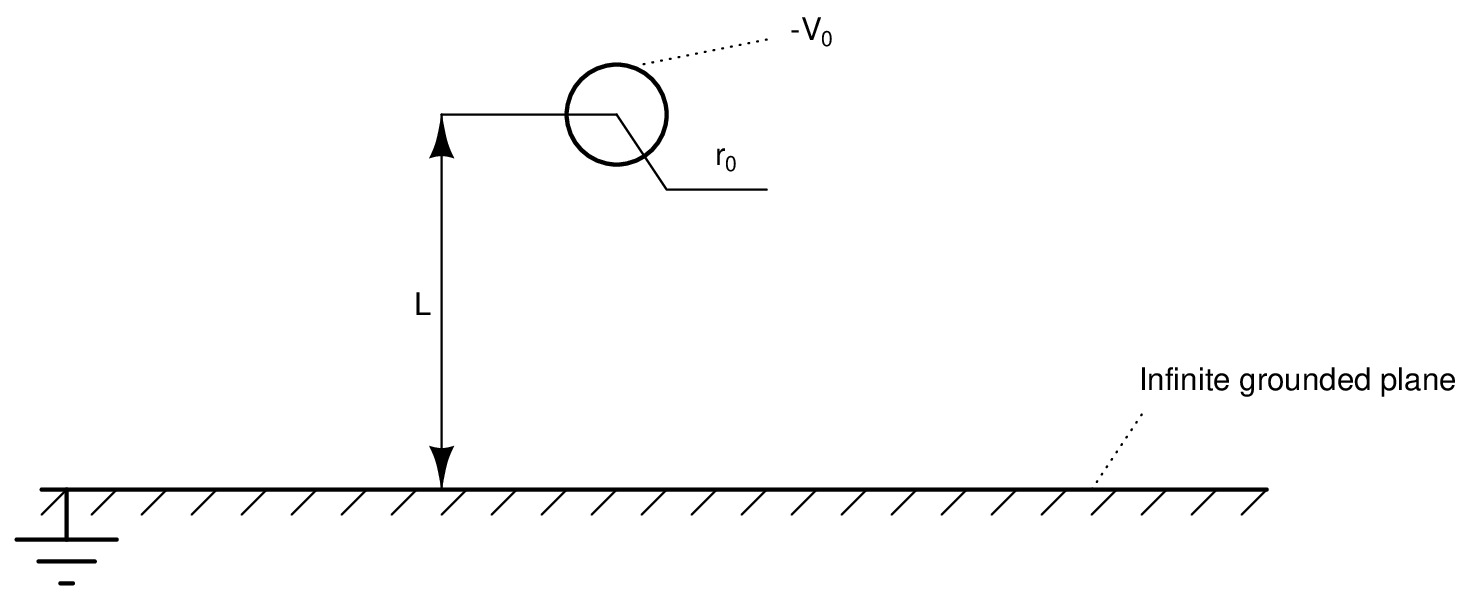
\includegraphics[width=0.5\textwidth]{images/IdealModel.jpg}
%    \caption{Model 1}\\\\
\begin{figure}[ht]
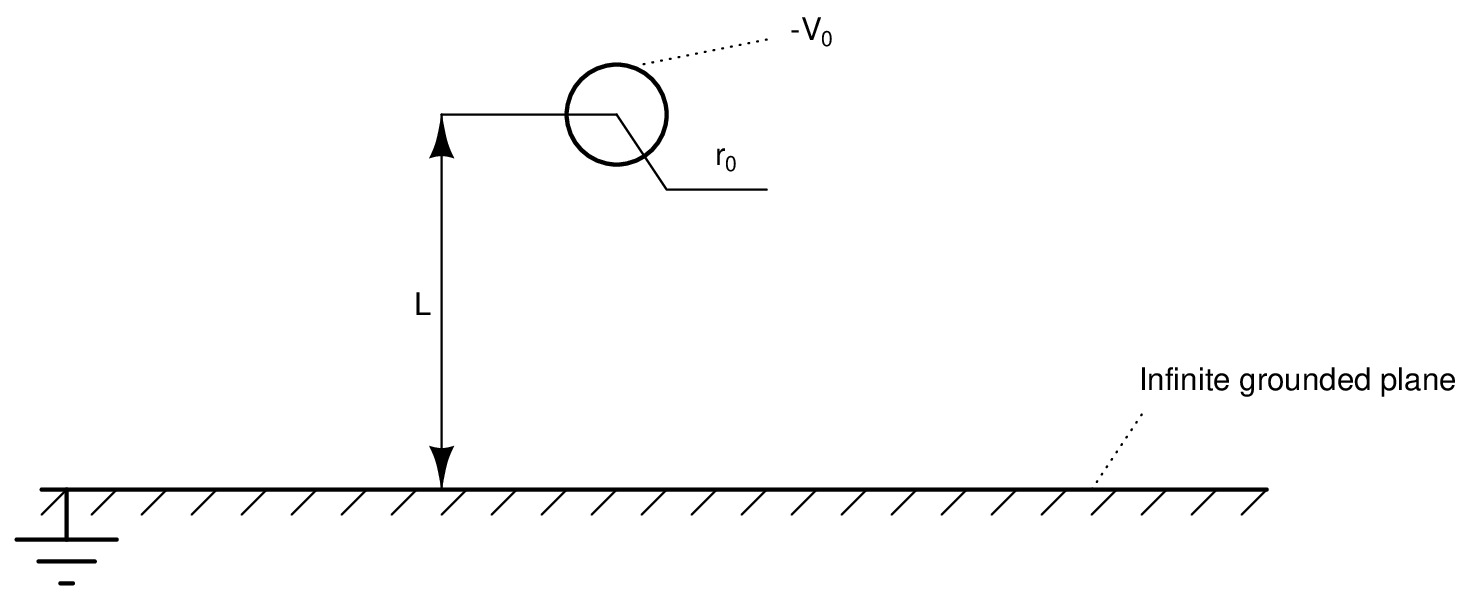
\includegraphics[width=0.5\textwidth]{images/IdealModel.jpg}
\caption{Model 1}
\end{figure}
To calculate the force exerted on the ions and the resulting thrust, we need to determine the electric field in different positions:
$$E = - \nabla V $$
This can be achieved by solving the Poisson equation\cite{sakr2}:
$$\nabla^2 V = - \frac{\rho_q }{\epsilon_o}$$
which relates the voltage distribution to the charge density. Since the considered region is charge-free and in a 2D cylindrical coordinate system, the Poisson equation simplifies accordingly to:
$$ \rho\frac{\partial^2 V}{\partial \rho^2}+ \rho^2\frac{\partial V}{\partial \rho} +\frac{\partial V}{\partial \phi}$$
with boundary conditions at $\rho < r_o , V=-V_o $  and $ \rho sin(\phi)=L$ , $ 0<\phi < \pi$  , $V=0$\\\\
\hspace{\parindent}As a result of the electric field and the ions resulting from the corona effect on the distance between the wire and the plate, there is a field with ions that make the gap conductor have terrible mobility and the current density flows from the wire into the plate under the governing equations 
$$\nabla \Vec{J} = 0$$
$$\Vec{J} = q(K_i \Vec{E} + \Vec{v}) - D\nabla q$$
Where D is the diffusion parameter and$ K_i$ is the ion mobility in the air at STP,
$K_io \approx 2 \times \frac{10^-4 m^2}{V.s} $\cite{sakr2}\\
$v(m/s)$ is the velocity of the ions in the air.
We can neglect the diffusion current and the velocity magnitude since $v$ is in the order of 4 to 6 (m/s) and q in order of $10^-19$\cite{sakr2}
$$\Vec{J} = qK_i\vec{E}$$
From the conservation of charge, we can get the charge in the system:
$$\nabla q \cdot \nabla \phi = -\frac{q^2}{\epsilon_o}$$
After this, we use both Navier-Stokes equations to get the velocity and pressure, assuming that the air is not compressed laminar flow and has a fixed pressure and viscosity.
$$\nabla \cdot \vec{u} = 0$$
$$\rho_f [\frac{\partial\Vec{u}}{\partial t} + (\Vec{u}\cdot \nabla) \Vec{u}] = -\nabla P + \nu \nabla^2 \vec{u} + q\vec{E}$$
After we get the pressure, it is required to know the airflow. Some parameters are required to be known: \\
1. Air dielectric strength is 3 times $10^6 V/m$.\\
2. From the above value, The smaller the $r_o$, the bigger the electric field intensity, as the smallest value we can get for $r_o$ without arching is 0.66 mm for the material 22 AWG.\\
3. The air density is 1.205 kg/m3.\\
4. Dynamic viscosity is 1.81 $\times 10^-5$ $kg/m.s$\\
5. Relative permittivity is 1\\
\subsection*{Model 2: wire to cylinder lifter}
% great habibi mehtag yebqa that elmodel altol
\hspace{\parindent}In this model, we deal with a more realistic model, so we focus on the charge density of the area in our equations, and this time we take into consideration the ionized region and use these equations to get the voltage.
\subsection*{Geometry of the model}
Our setup for the model consists of three main components:
•	Wire electrode\\
•	Aluminum foil electrode\\
•	The space between 2 electrodes (air)\\




%\begin{figure}[ht]
%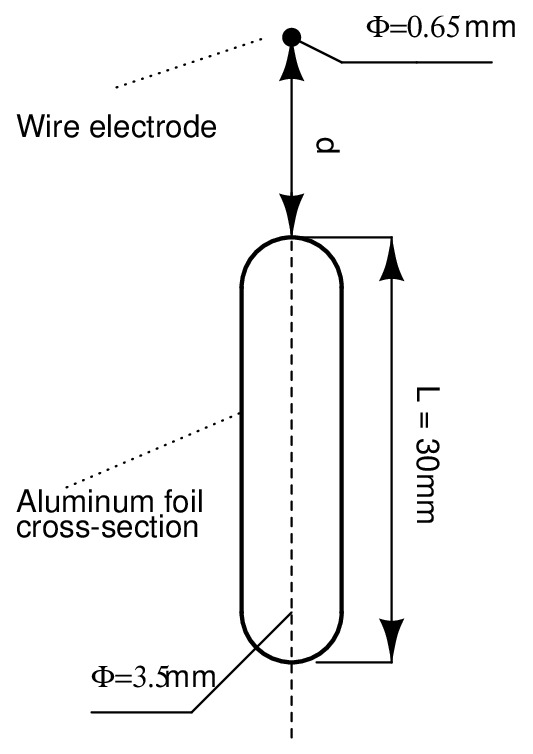
\includegraphics[width=0.5\textwidth]{images/cross-section.jpg}
%\caption{A cross-section of Model 2}
%\label{fig:cross-section}
%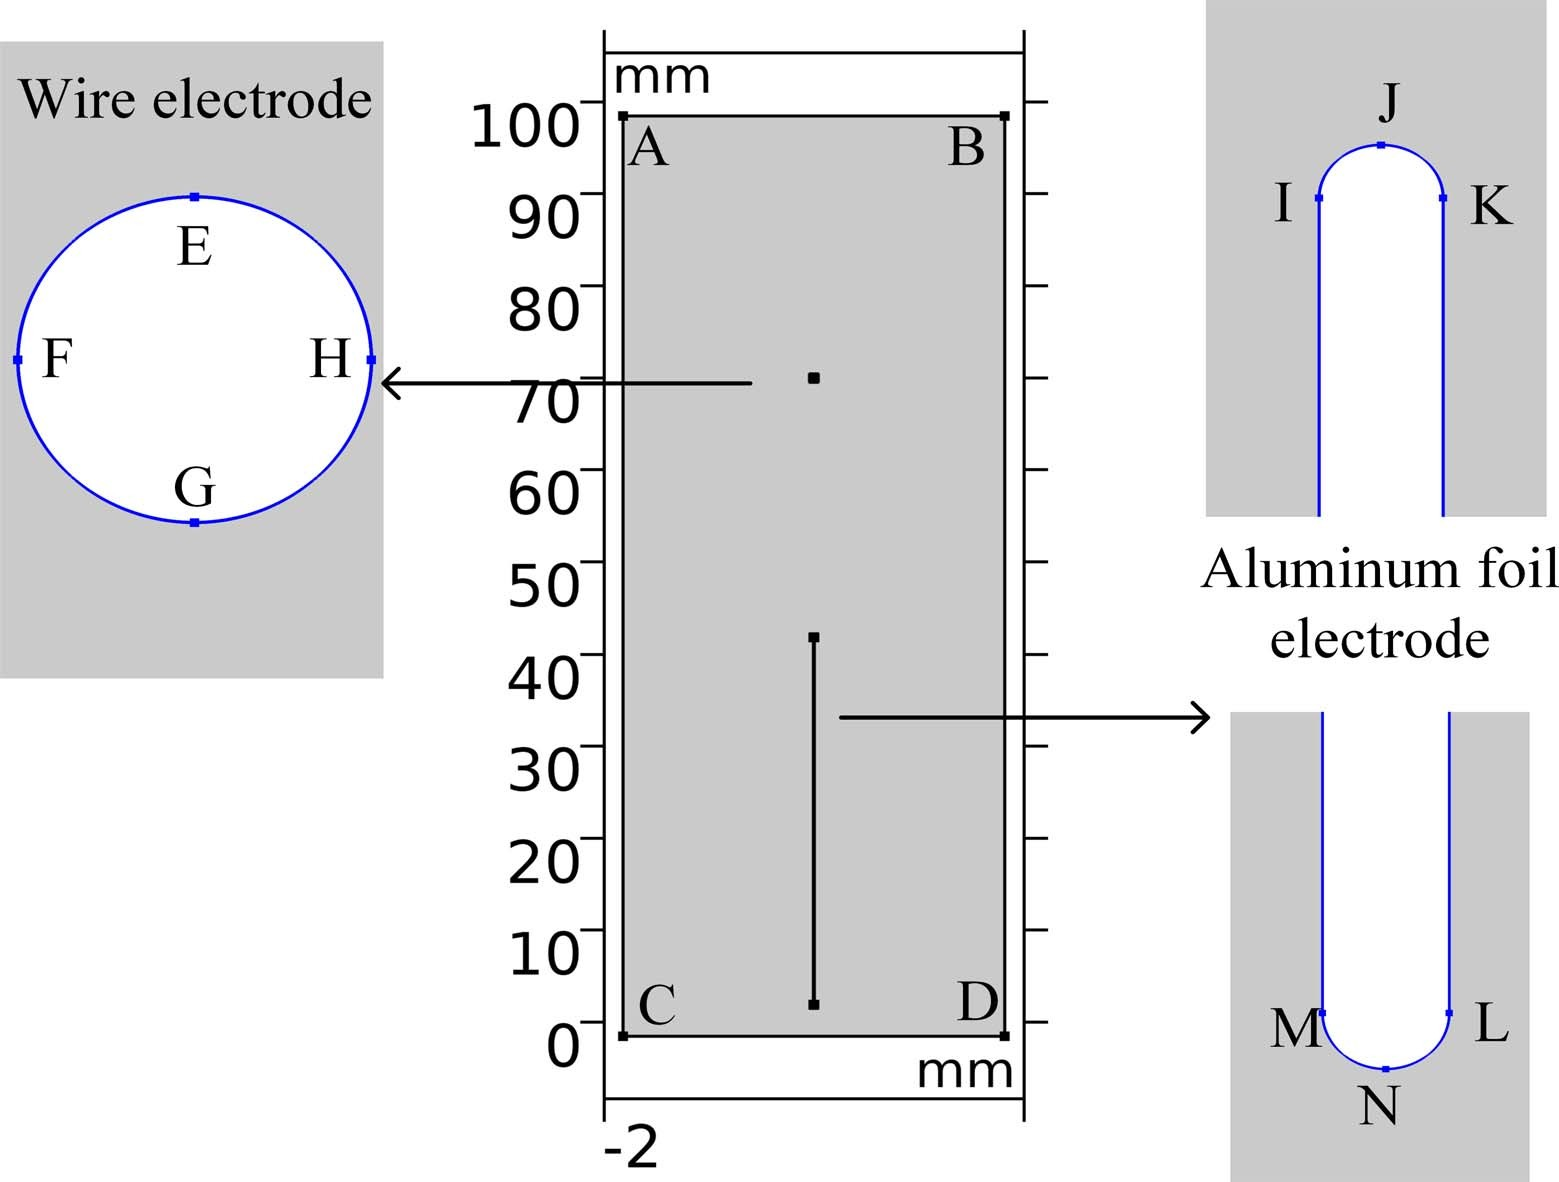
\includegraphics[width=0.5\textwidth]{images/neededimage.jpeg}
%\caption{ Model 2\cite{Elsalakawy}}% ok 
%\label{fig:model}
%\end{figure}fe figure kman lsa 3aiz a7th





\begin{figure}[ht]
    \centering
    \begin{subfigure}{.5\textwidth}
      \centering
      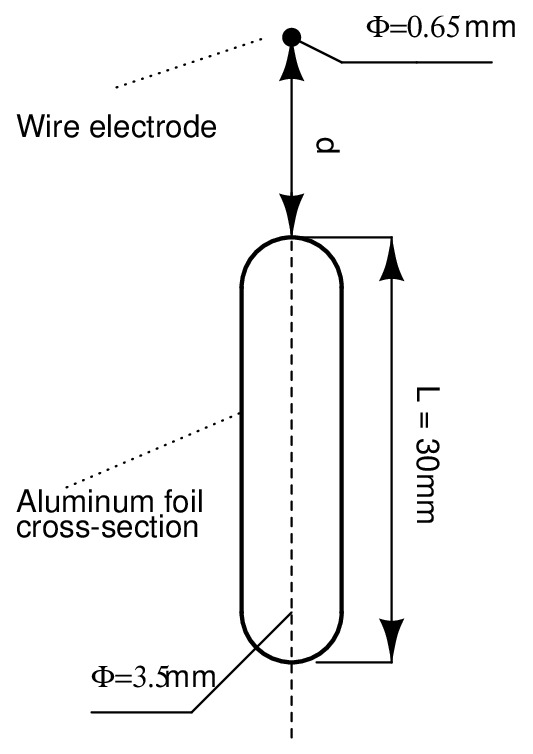
\includegraphics[width=.8\linewidth]{images/cross-section.jpg}
      \caption{A cross-section of Model 2}
    \end{subfigure}%
    \begin{subfigure}{.5\textwidth}
      \centering
      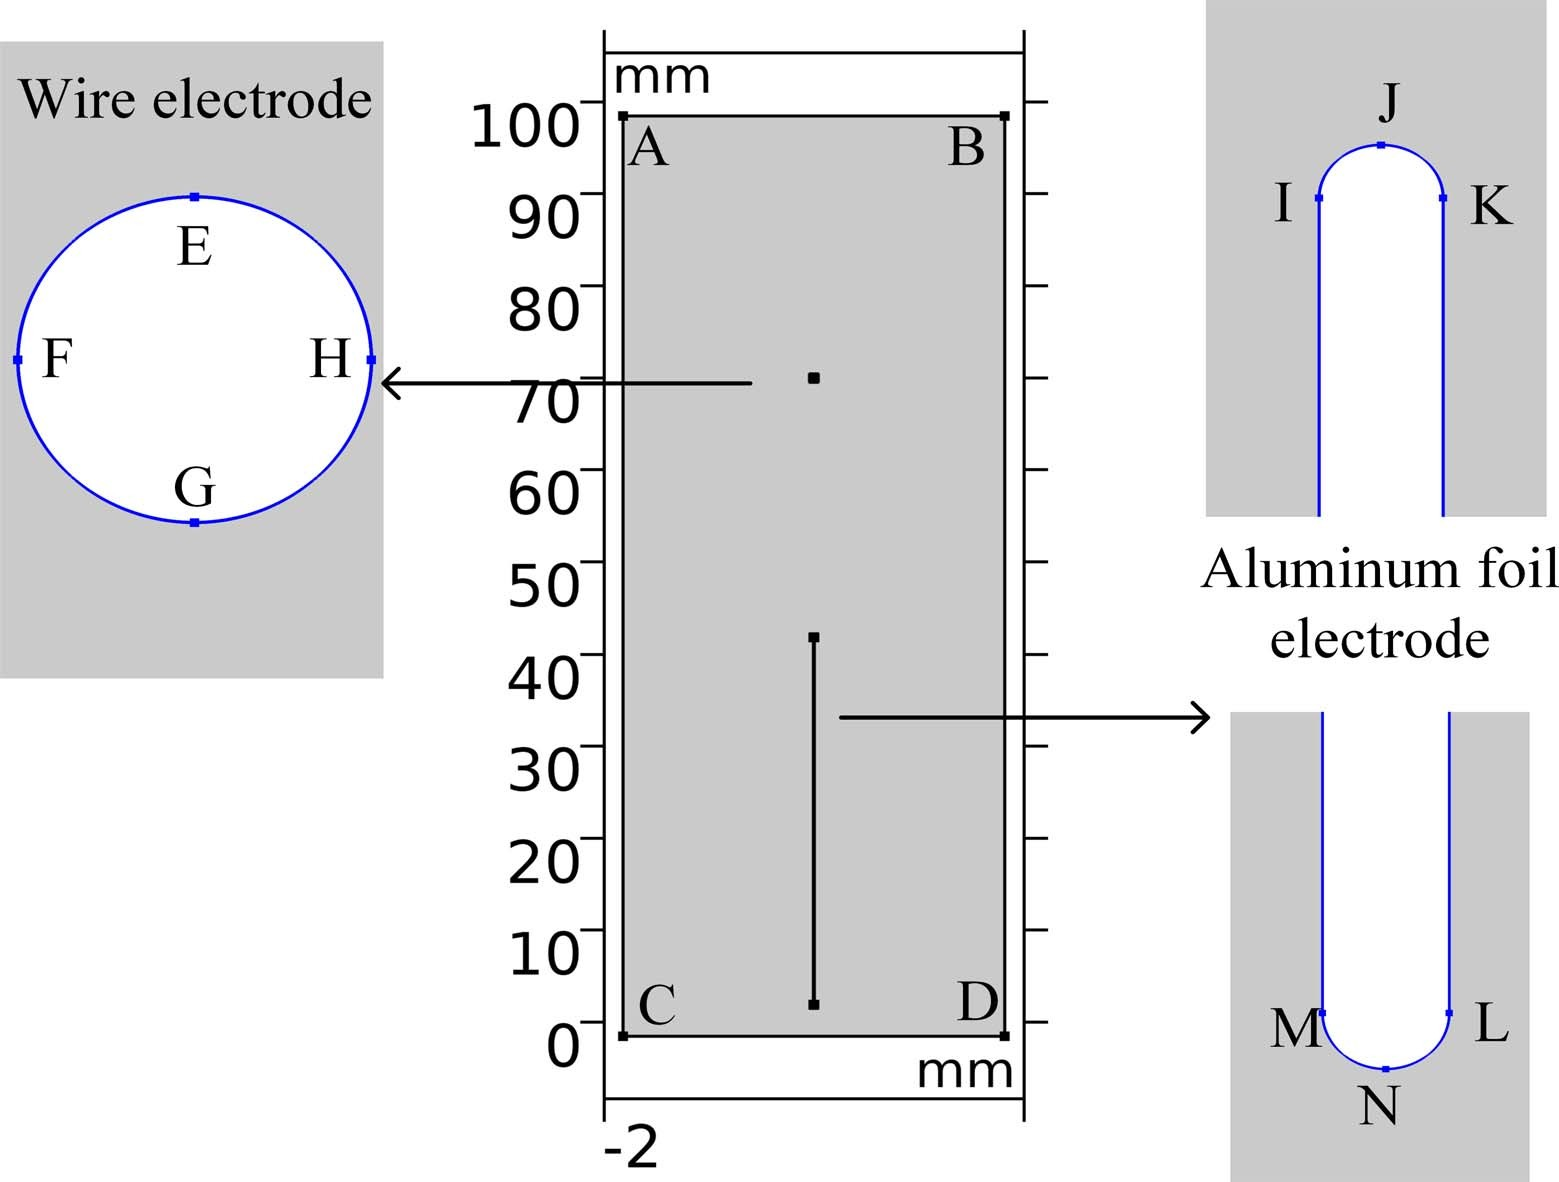
\includegraphics[width=1\linewidth]{images/neededimage.jpeg}
      \caption{ Model 2\cite{Elsalakawy}}
    \end{subfigure}
      \label{patents}
\end{figure}%3zeem





\subsection*{Assumptions}
There are some assumptions we take into consideration to model our problem:\\
•	the reduced electric field is   relatively low\\
•	conduction is superior to convection and ion diffusion\\
•	The fluid is incompressible laminar in the drift region. The incompressible flow decouples the energy conservation from the momentum equation\\
•	Fixed air \\
\subsection*{Governing Equations}
In our model we consider electrostatic interaction between electrodes and the space charges, the moment exchange, induced flow, the structural pressure, and viscous resistance.  
Three main equations govern our problem:\\
•	Navier stokes equations (conservation of mass and conservation of momentum)\\
•	Poisson equation\\
•	Current density equation\\
\subsection*{The Methodology}
1.	We use the Poisson equation to control the potential difference between two electrodes:
$$\nabla^2 V = - \frac{\rho_q }{\epsilon_o}$$
We can obtain the electric field between two electrodes from:
$$E = - \nabla V $$
2.	The current density Ji caused by the space charge in the drift region can be calculated as:
$$J_i = \mu_i E \rho_q + \rho_q u - D_i \nabla \rho_q$$
Where $\mu_i$ is the mobility of ions under the electric field, U(m/s) is the air velocity vector, and  
$D_i$ (m2/s) is the ion diffusion coefficient.
Since the reduced electric field is   relatively low,   $D_i$ can be approximately obtained by  
the following Einstein’s relationship:
$$D_i = \frac{\mu_i K_B T}{q}$$
3.	The charge density in the drift region can be calculated as:
$$\nabla \rho_q \cdot \nabla V - \frac{\rho_q^2}{\epsilon_o}=0$$
4.	Using Navier-Stokes equations (the mass continuity) to solve the fluid velocity
Under the condition of incompressible fluid:
$$\nabla u =0 $$
5.	Under the condition of direct current we can obtain air viscosity using:
\begin{align*}
F&= \rho_q E \\
&= -\rho_q\nabla V\end{align*}
6.	After solving for velocity and air viscosity we then use Navier–Stokes (the conservation of momentum) to solve for the pressure:
$$\rho(u\cdot \nabla)u= - \nabla p + \mu \nabla^2 u + \rho_q E$$
 The seven equations above are solved simultaneously to obtain physical quantities which describe our phenomena.\cite{Elsalakawy}
\subsection*{Boundary and Initial Conditions}
\subsubsection*{Assumptions:}
•	The thickness of the ionization region is ignored.\\
•	The electric field on the wire electrode surface remains unchanged when corona discharge starts.\\
•	The electric field intensity of corona discharge on the wire electrode can be determined using Peek's law.
\subsubsection*{Equations:}
1. Electric field strength on the surface of an ideal smooth cylindrical 
$$ E_p = E_o \delta\epsilon (1+ 0.308\sqrt{\delta r_c}) $$
  where:\\
* $E_p$ is the electric field strength (V/m)\\
* $E_o$ is the air breakdown electric strength $(3.31 × 10^6 V/m)$\\ \cite{Elsalakawy}
* $\delta$ is the relative air density (298 p/T)\\
* $r_c$ is the wire electrode radius (m)\\
* T is the temperature (293.15 K)\\
* p is the pressure (1 atm)\\\\
2. Surface charge density:
$$\sigma = \epsilon E_p$$
where:\\
* $\sigma$ is the surface charge density (C/m²)\\
* $\epsilon$ is the electrode's dimensionless surface roughness (1 for a smooth surface)\\\\
3. Electric field in the ionization region:
$$E(r) = \frac{E_p r_c}{r} $$
where:\\
* E(r) is the electric field at radial position r (V/m)\\
* r is the radial position (m)\\
* $r_c$ is the wire electrode radius (m)\\\\
4. Ionization region radius:
$$ r_i = r_c \delta (1+ 0.308\sqrt{\delta r_c}) $$
where:\\
* $r_i$ is the ionization region radius (m)\\\\
5. Voltage applied to the wire electrode surface:
$$V_i = V_c - E_p r_c \ln{(\frac{E_p}{E_o})}$$
where:\\
* $V_i$ is the voltage applied to the wire electrode surface (V)\\
* $V_c$ is the voltage planned to be applied to the wire electrode (V)\\


